\documentclass[12pt,a4paper]{article}
\usepackage[utf8]{inputenc}
\usepackage{amsmath,amssymb,amsthm}
\usepackage{geometry}
\usepackage{graphicx}
\usepackage{hyperref}
\usepackage{enumitem}
\usepackage{xcolor}
\usepackage{tcolorbox}
\tcbuselibrary{breakable,skins}
\usepackage{mathtools}
\usepackage{fancyhdr}
\usepackage{tikz}
\usepackage{pgfplots}
\pgfplotsset{compat=1.18}
\usetikzlibrary{arrows.meta,positioning,calc,patterns,decorations.pathreplacing,shapes}

\geometry{margin=1in}

\pagestyle{fancy}
\fancyhf{}
\rhead{Machine Learning Foundations}
\lhead{Detailed Notes}
\cfoot{\thepage}

\title{\textbf{Machine Learning Foundations: \\ From Geometry to Classification}}
\author{Akshay Redekar}
\date{\today}

\newtheoremstyle{directpoint}
  {}% Space above
  {}% Space below
  {}% Body font
  {}% Indent amount
  {\bfseries}% Theorem head font
  {}% Punctuation after theorem head
  {\newline}% Space after theorem head
  {\thmnote{#3}}% Theorem head spec

\theoremstyle{directpoint}
\newtheorem*{definition}{Definition}

\theoremstyle{definition}
\newtheorem{theorem}{Theorem}[section]
\newtheorem{example}{Example}[section]
\newtheorem{problem}{Problem}[section]
\newtheorem{property}{Property}[section]

\definecolor{highlight}{RGB}{255,255,200}

% Add page border using tikz
\AddToHook{shipout/background}{%
    \begin{tikzpicture}[remember picture, overlay]
        \draw[line width=0.5pt]
            ($(current page.north west) + (0.2in,-0.2in)$)
            rectangle
            ($(current page.south east) + (-0.2in,0.2in)$);
    \end{tikzpicture}
}

\begin{document}

\maketitle
\tableofcontents
\newpage

\section{Introduction: Machine Learning Context}

\subsection{Module Overview}

This module represents the last foundations component before building your first machine learning model. The primary goal is to understand the mathematical principles that enable machines to learn from data. The module spans approximately 10 lectures over one month and covers four core mathematical topics essential for machine learning.

\textbf{Core Topics:}
\begin{itemize}
    \item Coordinate Geometry - Understanding how to represent data spatially
    \item Linear Algebra - Vector operations and transformations
    \item Calculus - Optimization through derivatives and gradients
    \item Optimization - Finding the best model parameters
\end{itemize}

\textbf{Learning Flow:} The pedagogy follows a systematic progression from abstract concepts to concrete implementations. Each topic moves through: Concepts $\rightarrow$ Visualizations $\rightarrow$ Mathematics $\rightarrow$ Code. This approach ensures both theoretical understanding and practical implementation skills.

\subsection{Class Structure and Expectations}

\textbf{Class 1 Approach:} The first class takes a deliberate, measured pace. It introduces machine learning through practical examples and emphasizes geometric intuition before diving into formal mathematics. Key focus areas include visualization techniques and fundamental equations, particularly the equation of a line which serves as the foundation for linear decision boundaries.

\textbf{Subsequent Classes:} Starting from Class 2, the material becomes more rigorous with heavier emphasis on mathematical formalism and geometric interpretations. This progression allows students to build intuition first before tackling more complex mathematical frameworks.

\subsection{Why Study Machine Learning?}

Machine learning enables computers to make decisions and predictions without being explicitly programmed with every possible rule. Instead of writing thousands of conditional statements, we can train models to discover patterns in data automatically. This capability has applications ranging from industrial automation to predictive analytics.

\textbf{Real-World Applications Include:}
\begin{itemize}
    \item Quality control and sorting in manufacturing
    \item Predictive modeling in sports and entertainment
    \item Medical diagnosis and healthcare analytics
    \item Financial forecasting and risk assessment
    \item Natural language processing and computer vision
\end{itemize}

\newpage

\section{Classification: The Fruit Sorting Problem}

\subsection{Problem Statement}

Consider an assembly line at an orange juice factory that processes both oranges and tangerines. Currently, a human worker examines each fruit passing through a scanner and manually operates a separator to direct fruits into the appropriate bins. Our goal is to replace this manual process with an automated algorithm that can classify each fruit correctly.

\begin{center}
\resizebox{\textwidth}{!}{%
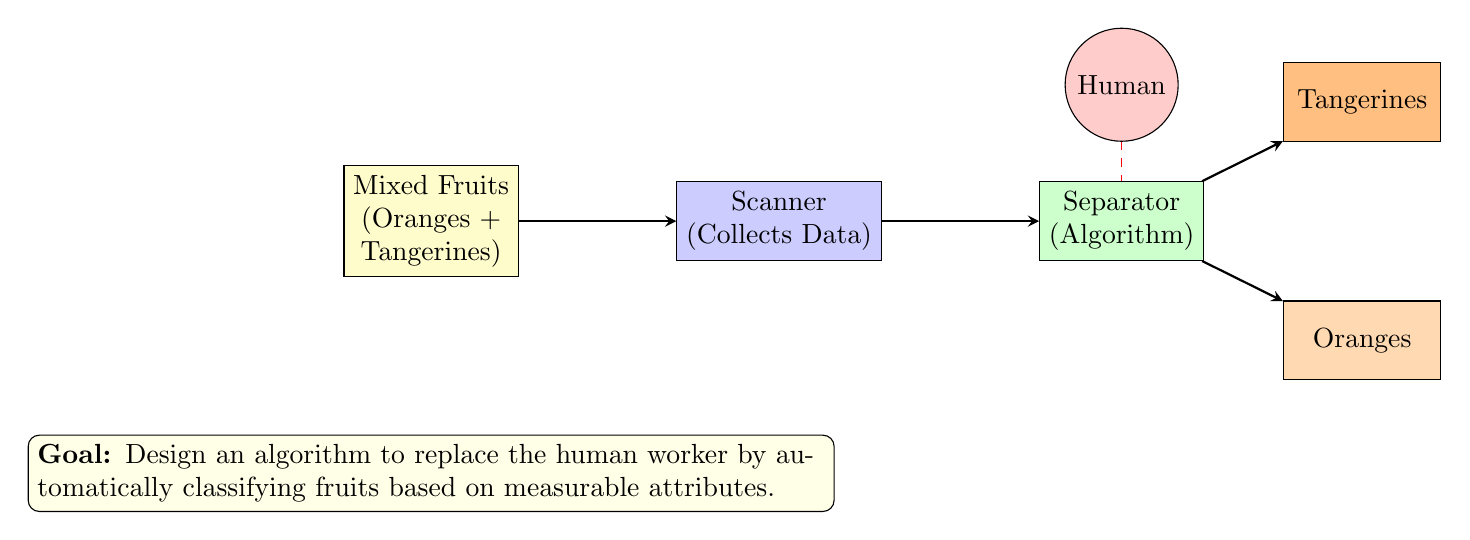
\begin{tikzpicture}[
    node distance=2cm,
    box/.style={rectangle, draw, minimum width=2cm, minimum height=1cm, align=center},
    arrow/.style={->, >=stealth, thick}
]
    % Input
    \node[box, fill=yellow!20] (input) {Mixed Fruits\\(Oranges +\\Tangerines)};
    
    % Scanner
    \node[box, fill=blue!20, right=of input] (scanner) {Scanner\\(Collects Data)};
    
    % Separator (with human)
    \node[box, fill=green!20, right=of scanner] (separator) {Separator\\(Algorithm)};
    
    % Human (to be replaced)
    \node[draw, circle, above=0.5cm of separator, fill=red!20] (human) {Human};
    \draw[dashed, red] (human) -- (separator);
    
    % Outputs
    \node[box, fill=orange!30, below right=0.5cm and 1cm of separator] (oranges) {Oranges};
    \node[box, fill=orange!50, above right=0.5cm and 1cm of separator] (tangerines) {Tangerines};
    
    % Arrows
    \draw[arrow] (input) -- (scanner);
    \draw[arrow] (scanner) -- (separator);
    \draw[arrow] (separator) -- (oranges);
    \draw[arrow] (separator) -- (tangerines);
    
    % Goal annotation
    \node[below=2cm of input, text width=10cm, align=left, draw, fill=yellow!10, rounded corners] {
        \textbf{Goal:} Design an algorithm to replace the human worker by automatically classifying fruits based on measurable attributes.
    };
\end{tikzpicture}%
}
\end{center}

\subsection{Feature Selection}

The first critical step in any machine learning problem is identifying which attributes (features) are useful for making predictions. Not all measurable properties are equally informative for classification.

\textbf{Question:} Which attributes might help distinguish oranges from tangerines?

\textbf{Analysis of Potential Features:}
\begin{itemize}
    \item \textbf{Diameter:} (Valid) Useful - Can be collected from the scanner. Oranges and tangerines typically have different size distributions.
    \item \textbf{Weight:} (Valid) Useful - Can be collected from the scanner. Weight correlates with size and density differences between the two fruits.
    \item \textbf{Color:} (Invalid) Not useful - Both fruits are orange-colored, making color a poor discriminator for this specific classification task.
\end{itemize}

This feature selection process demonstrates an important principle: effective machine learning requires domain knowledge to identify which measurements contain discriminative information.

\subsection{Essential Terminology}

Before proceeding further, we must establish precise definitions for the key concepts used throughout machine learning.

\begin{definition}[Features]
Features (also called independent variables, attributes, or predictors) are the input variables used to make predictions. In our fruit sorting example, the features are Diameter (D) and Weight (W). Features are denoted as $\mathbf{x} = [x_1, x_2, \ldots, x_d]^T$ where $d$ is the number of features.
\end{definition}

\begin{definition}[Target]
The target (also called the dependent variable or label) is the output we want to predict. In our example, the target is the fruit type (F), which can be either Orange (O) or Tangerine (T). The target is typically denoted as $y$.
\end{definition}

\begin{definition}[Data Point]
A data point is a single observation consisting of feature values and the corresponding target value. For example, (10, 80, O) represents a fruit with diameter 10, weight 80, which is an orange.
\end{definition}

\begin{definition}[Dataset]
A dataset is a collection of many data points. We typically denote a dataset as $\mathcal{D} = \{(\mathbf{x}_i, y_i)\}_{i=1}^{n}$ where $n$ is the number of examples.
\end{definition}

\textbf{Example Dataset:}

\begin{center}
\begin{tabular}{|c|c|c|}
\hline
\textbf{Diameter (D)} & \textbf{Weight (W)} & \textbf{Fruit (F)} \\
\hline
10 & 100 & T \\
8 & 70 & O \\
10 & 80 & O \\
7 & 100 & T \\
9 & 85 & O \\
11 & 95 & T \\
\hline
\end{tabular}
\end{center}

\subsection{The Challenge of Manual Rules}

One might initially attempt to solve this classification problem by writing explicit rules. For instance: "If weight $> 90$, then Tangerine; otherwise Orange" or "If diameter $< 8$, then Orange; otherwise Tangerine."

\textbf{Problems with Manual Rules:}
\begin{itemize}
    \item \textbf{Threshold Calibration:} Determining the exact threshold values (like 90 for weight) is difficult and requires extensive trial and error.
    \item \textbf{Multiple Features:} When combining multiple features, the rule complexity grows exponentially. How do we balance diameter and weight together?
    \item \textbf{Rigidity:} Manual rules don't adapt when new data arrives. If fruit sizes change seasonally, rules must be manually updated.
    \item \textbf{Scalability:} With more features (texture, acidity, sugar content), manual rule creation becomes impractical.
\end{itemize}

This motivates the need for a more systematic, mathematical approach to classification.

\newpage

\section{Geometric Visualization of Classification}

\subsection{The Cartesian Plane Representation}

Rather than thinking in terms of discrete rules, we can visualize the classification problem geometrically. Each data point can be represented as a coordinate in a Cartesian plane where the x-axis represents Diameter (D) and the y-axis represents Weight (W).

\begin{center}
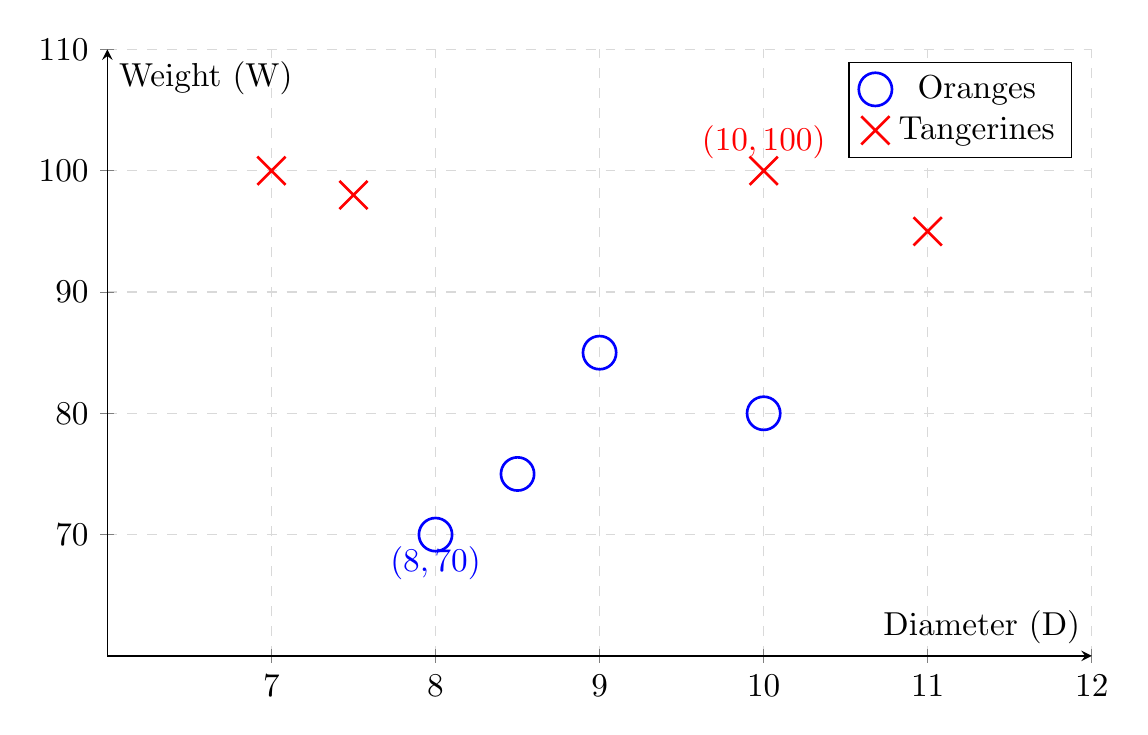
\begin{tikzpicture}[scale=1.2]
    \begin{axis}[
        axis lines=middle,
        xlabel={Diameter (D)},
        ylabel={Weight (W)},
        xmin=6, xmax=12,
        ymin=60, ymax=110,
        width=12cm,
        height=8cm,
        grid=major,
        grid style={dashed, gray!30}
    ]
    
    % Orange points (circles)
    \addplot[only marks, mark=o, mark size=5pt, blue, thick] coordinates {
        (8, 70)
        (10, 80)
        (9, 85)
        (8.5, 75)
    };
    
    % Tangerine points (crosses)
    \addplot[only marks, mark=x, mark size=6pt, red, thick] coordinates {
        (10, 100)
        (7, 100)
        (11, 95)
        (7.5, 98)
    };
    
    % Example point annotation
    \node[blue, below] at (axis cs:8,70) {$(8, 70)$};
    \node[red, above] at (axis cs:10,100) {$(10, 100)$};
    
    % Legend
    \legend{Oranges, Tangerines}
    \end{axis}
\end{tikzpicture}
\end{center}

\textbf{Key Observation:} When plotted geometrically, the two classes of fruits form distinct clusters. Oranges tend to occupy one region of the feature space, while tangerines occupy another. This spatial separation is the foundation of classification algorithms.

\subsection{Finding a Separation Boundary}

\textbf{Question:} Looking at the scatter plot above, can you think of a geometric way to separate these two groups of points?

\textbf{Answer:} A straight line!

We can draw a line that separates the orange points from the tangerine points. Any new fruit that appears can then be classified based on which side of the line it falls on.

\begin{center}
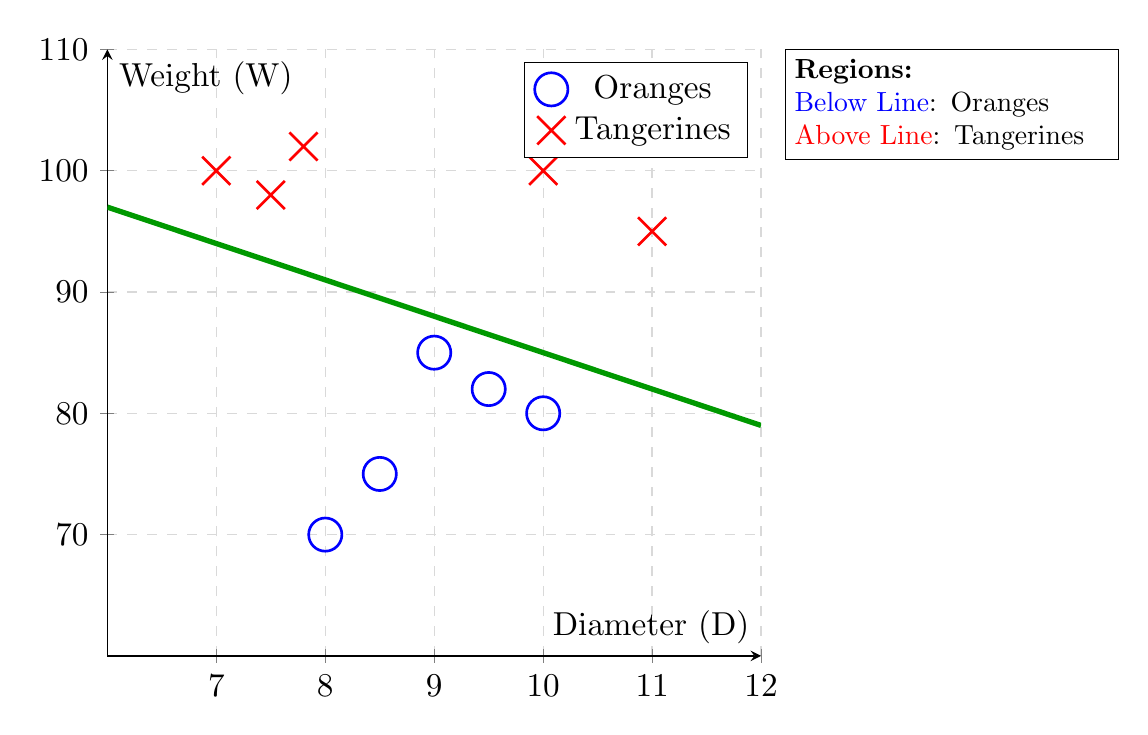
\begin{tikzpicture}[scale=1.2]
    \begin{axis}[
        axis lines=middle,
        xlabel={Diameter (D)},
        ylabel={Weight (W)},
        xmin=6, xmax=12,
        ymin=60, ymax=110,
        width=8.5cm,
        height=8cm,
        grid=major,
        grid style={dashed, gray!30}
    ]
    
    % Orange points
    \addplot[only marks, mark=o, mark size=5pt, blue, thick] coordinates {
        (8, 70) (10, 80) (9, 85) (8.5, 75) (9.5, 82)
    };
    
    % Tangerine points
    \addplot[only marks, mark=x, mark size=6pt, red, thick] coordinates {
        (10, 100) (7, 100) (11, 95) (7.5, 98) (7.8, 102)
    };
    
    % Decision boundary line
    \addplot[green!60!black, ultra thick, domain=6:12] {-3*x + 115};
    \addlegendentry{Decision Boundary}

    % Region labels - moved to legend or removed if obvious from context, 
    % but user wants side legend. Let's add them as dummy plots or just clean up.
    % Actually, for regions, let's keep them if they don't overlap, but the user complaint suggests they might.
    % Let's use a side legend node for regions description.
    
    \legend{Oranges, Tangerines}
    \end{axis}
    
    % Side Legend for Regions
    \node[draw, fill=white, align=left, anchor=north west, text width=4cm] at (current axis.north east) [xshift=0.3cm] {
        \textbf{Regions:}\\
        \textcolor{blue}{Below Line}: Oranges\\
        \textcolor{red}{Above Line}: Tangerines
    };
\end{tikzpicture}
\end{center}

\subsection{Core Machine Learning Definitions}

\begin{definition}[Decision Boundary]
A decision boundary is a geometric surface (line in 2D, plane in 3D, hyperplane in higher dimensions) that separates different classes in the feature space. Points on one side of the boundary are classified as one class, while points on the other side belong to the other class.
\end{definition}

\begin{definition}[Misclassification]
A misclassified point is a data point that falls on the wrong side of the decision boundary. For example, if an orange appears in the tangerine region, it represents a classification error.
\end{definition}

\begin{definition}[Machine Learning]
Machine learning is the ability of a computer system to automatically find the optimal decision boundary by "learning" from the given dataset, rather than having the boundary defined manually through hard-coded rules.
\end{definition}

\subsection{Extension: Multiple Classes and Complex Boundaries}

While our fruit sorting example involves only two classes (binary classification), real-world problems often involve multiple categories. For instance, classifying fruits into apples, oranges, tangerines, and lemons would require multiple decision boundaries.

\textbf{Important Considerations:}
\begin{itemize}
    \item The number of classes or labels can exceed two, requiring more sophisticated boundary configurations.
    \item Decision boundaries need not be straight lines - they can be curves, circles, or complex shapes depending on how the data is distributed.
    \item The choice of boundary shape impacts both model accuracy and computational complexity.
\end{itemize}

\begin{center}
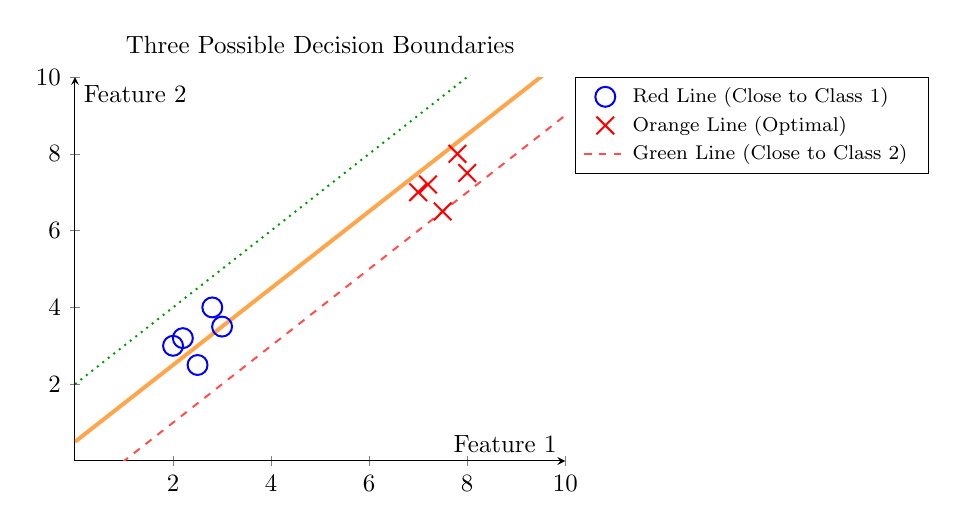
\begin{tikzpicture}[scale=0.9]
    \begin{axis}[
        axis lines=middle,
        xlabel={Feature 1},
        ylabel={Feature 2},
        xmin=0, xmax=10,
        ymin=0, ymax=10,
        width=8.5cm,
        height=7cm,
        title={Three Possible Decision Boundaries},
        legend style={at={(1.02,1)}, anchor=north west, font=\footnotesize, nodes={text width=4cm, align=left}}
    ]
    
    % Class 1 (blue circles)
    \addplot[only marks, mark=o, mark size=4pt, blue, thick] coordinates {
        (2, 3) (2.5, 2.5) (3, 3.5) (2.8, 4) (2.2, 3.2)
    };
    
    % Class 2 (red crosses)
    \addplot[only marks, mark=x, mark size=5pt, red, thick] coordinates {
        (7, 7) (7.5, 6.5) (8, 7.5) (7.8, 8) (7.2, 7.2)
    };
    
    % Three different boundary options
    \addplot[red!70, thick, dashed, domain=0:10] {x - 1};
    \addlegendentry{Red Line (Close to Class 1)}
    
    \addplot[orange!70, ultra thick, domain=0:10] {x + 0.5};
    \addlegendentry{Orange Line (Optimal)}
    
    \addplot[green!60!black, thick, dotted, domain=0:10] {x + 2};
    \addlegendentry{Green Line (Close to Class 2)}
    
    \end{axis}
\end{tikzpicture}
\end{center}

\textbf{Critical Question:} Which line is the "best" decision boundary?

\textbf{Answer:} The orange line represents the optimal boundary because it maintains the maximum distance from both classes. This concept of maximizing the margin between classes is fundamental to support vector machines and robust classification.

\subsection{Practical Example: IPL Win Prediction}

To further illustrate classification, consider predicting cricket match outcomes for the Indian Premier League (IPL). A marketing company needs to decide when to stop an advertising campaign based on match progress.

\textbf{Dataset Structure:}
\begin{itemize}
    \item \textbf{Features:} Runs scored, Overs completed
    \item \textbf{Target:} Outcome (Win or Loss)
\end{itemize}

When visualized as a scatter plot with Runs on one axis and Overs on the other, winning matches cluster in one region while losing matches cluster elsewhere. A decision boundary can separate these regions, allowing the system to predict match outcomes in real-time and trigger marketing decisions accordingly.

\newpage

\section{Mathematical Foundations: The Equation of a Line}

\subsection{What is a Line Mathematically?}

In coordinate geometry, a line represents all points that satisfy a specific linear relationship between coordinates. The most intuitive form is the slope-intercept equation.

\begin{definition}[Slope-Intercept Form]
The slope-intercept form of a line is given by:
\begin{equation}
y = mx + c
\end{equation}
where:
\begin{itemize}
    \item $m$ is the slope (gradient) - measures the steepness of the line
    \item $c$ is the y-intercept - the point where the line crosses the y-axis
\end{itemize}
\end{definition}

\begin{center}
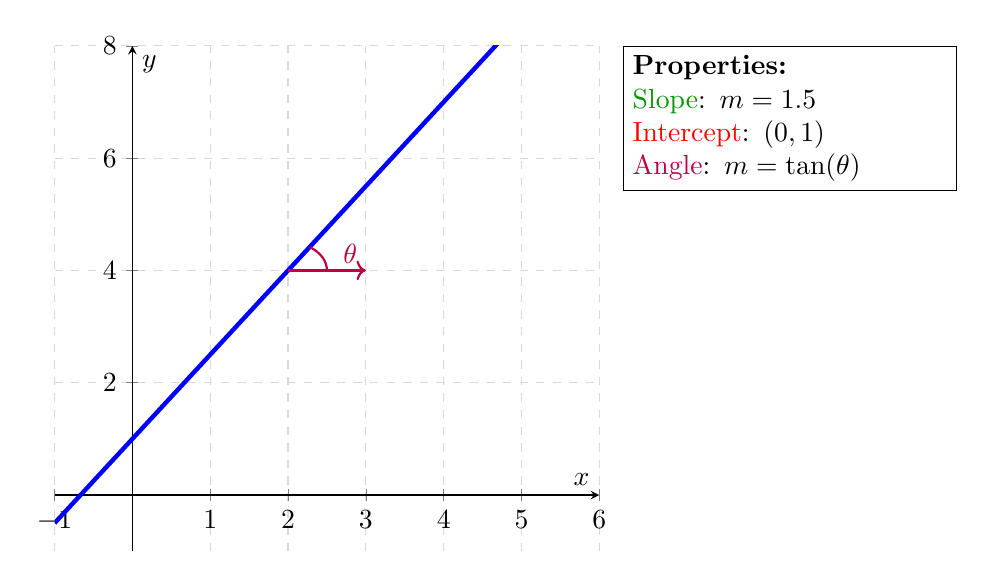
\begin{tikzpicture}
    \begin{axis}[
        axis lines=middle,
        xlabel=$x$,
        ylabel=$y$,
        xmin=-1, xmax=6,
        ymin=-1, ymax=8,
        width=8.5cm,
        height=8cm,
        grid=major,
        grid style={dashed, gray!30}
    ]
    
    % Line y = 1.5x + 1
    \addplot[blue, ultra thick, domain=-1:5] {1.5*x + 1};
    
    % Angle
    \draw[thick, purple, ->] (axis cs:2,4) -- (axis cs:3,4);
    \draw[thick, purple] (axis cs:2.5,4) arc (0:56:0.5);
    \node[purple] at (axis cs:2.8,4.3) {$\theta$};
    
    \end{axis}
    
    % Side Legend for properties
    \node[draw, fill=white, align=left, anchor=north west, text width=4cm] at (current axis.north east) [xshift=0.3cm] {
        \textbf{Properties:}\\
        \textcolor{green!60!black}{Slope}: $m = 1.5$\\
        \textcolor{red}{Intercept}: $(0, 1)$\\
        \textcolor{purple}{Angle}: $m = \tan(\theta)$
    };
\end{tikzpicture}
\end{center}

\subsection{Understanding Slope}

The slope quantifies how much $y$ changes for a unit change in $x$. It can be computed using any two points on the line.

\begin{property}[Slope Formula]
For any two points $(x_1, y_1)$ and $(x_2, y_2)$ on a line:
\begin{equation}
m = \frac{\Delta y}{\Delta x} = \frac{y_2 - y_1}{x_2 - x_1}
\end{equation}
\end{property}

\textbf{Relationship to Angle:} The slope is also related to the angle $\theta$ that the line makes with the positive x-axis:
\begin{equation}
m = \tan(\theta) \quad \text{or equivalently} \quad \theta = \tan^{-1}(m)
\end{equation}

\begin{example}[Identifying Linear Relationships]
\textbf{Problem 1:} Given points $(1, 2), (2, 4), (3, 6), (4, 8)$, what is the equation of the line?

\textbf{Solution:} 
Computing the slope using first two points:
\begin{equation}
m = \frac{4 - 2}{2 - 1} = \frac{2}{1} = 2
\end{equation}

Finding the y-intercept using point $(1, 2)$:
\begin{equation}
2 = 2(1) + c \implies c = 0
\end{equation}

\textbf{Answer:} $y = 2x$

\textbf{Problem 2:} Given points with a flatter slope that pass through $(0, 2)$ and $(1, 3)$, find the equation.

\textbf{Solution:}
\begin{equation}
m = \frac{3 - 2}{1 - 0} = 1
\end{equation}

The y-intercept is clearly $c = 2$ (given that the line passes through $(0, 2)$).

\textbf{Answer:} $y = x + 2$
\end{example}

\subsection{Parallel Lines}

\begin{property}[Parallel Lines]
Two lines are parallel if and only if they have the same slope but different y-intercepts:
\begin{equation}
l_1 \parallel l_2 \iff m_1 = m_2 \text{ and } c_1 \neq c_2
\end{equation}
\end{property}

\begin{center}
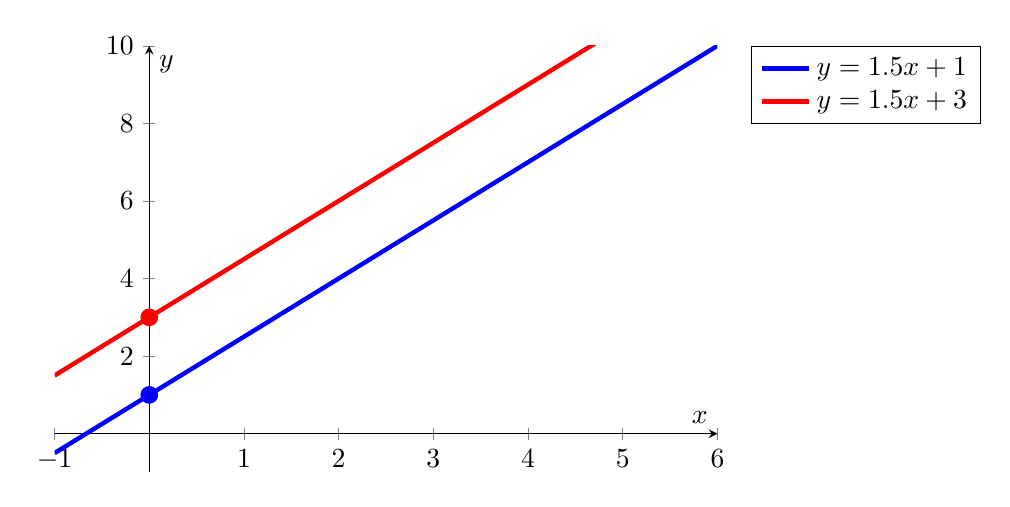
\begin{tikzpicture}
    \begin{axis}[
        axis lines=middle,
        xlabel=$x$,
        ylabel=$y$,
        xmin=-1, xmax=6,
        ymin=-1, ymax=10,
        width=10cm,
        height=7cm,
        legend style={at={(1.05,1)}, anchor=north west}
    ]
    
    % First line: y = 1.5x + 1
    \addplot[blue, ultra thick, domain=-1:6] {1.5*x + 1};
    \addlegendentry{$y = 1.5x + 1$}
    
    % Second line: y = 1.5x + 3
    \addplot[red, ultra thick, domain=-1:6] {1.5*x + 3};
    \addlegendentry{$y = 1.5x + 3$}
    
    % Intercepts
    \addplot[mark=*, mark size=3pt, blue] coordinates {(0, 1)};
    \addplot[mark=*, mark size=3pt, red] coordinates {(0, 3)};
    
    \end{axis}
\end{tikzpicture}
\end{center}

\textbf{Note:} Parallel lines never intersect because they maintain the same angle with the x-axis throughout.

\begin{example}[Parallel Lines Problem]
\textbf{Question:} Find the value of $m$ if the line $y = mx + 3$ is parallel to $0.5y - x = 0$.

\textbf{Solution:} First, convert the second equation to slope-intercept form:
\begin{align}
0.5y - x &= 0 \\
0.5y &= x \\
y &= 2x
\end{align}

The slope of the second line is $m_2 = 2$. For the lines to be parallel, we need:
\begin{equation}
m_1 = m_2 = 2
\end{equation}

\textbf{Answer:} $m = 2$
\end{example}

\subsection{Perpendicular Lines}

\begin{property}[Perpendicular Lines]
Two lines are perpendicular if and only if the product of their slopes equals $-1$:
\begin{equation}
l_1 \perp l_2 \iff m_1 \cdot m_2 = -1 \iff m_1 = -\frac{1}{m_2}
\end{equation}
\end{property}

\textbf{Significance for Machine Learning:} The distance from a point to a line is measured along the perpendicular direction. Understanding perpendicular lines is therefore crucial for computing classification margins and distances.

\begin{center}
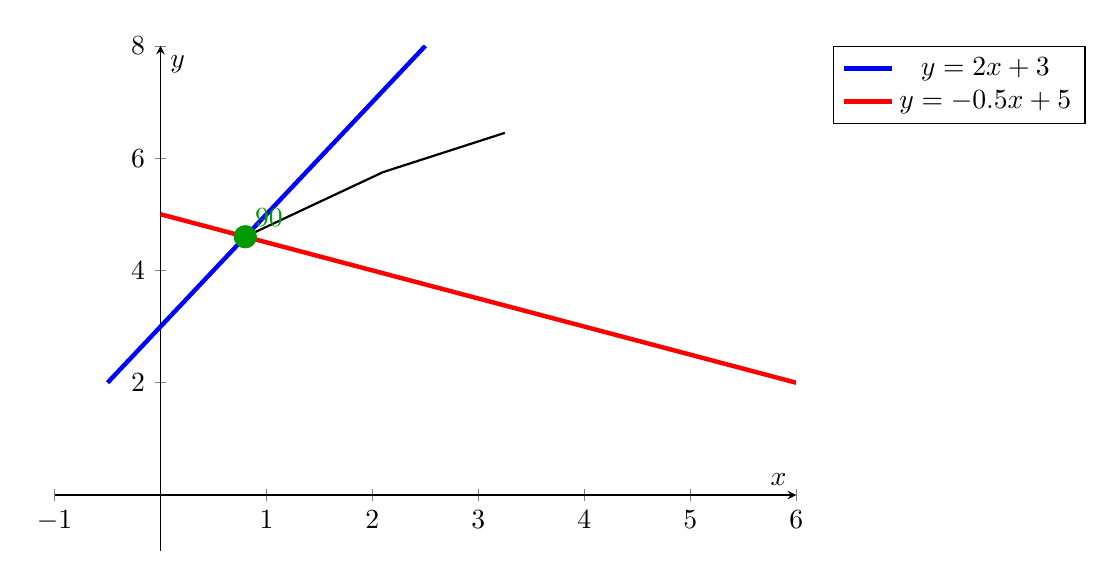
\begin{tikzpicture}
    \begin{axis}[
        axis lines=middle,
        xlabel=$x$,
        ylabel=$y$,
        xmin=-1, xmax=6,
        ymin=-1, ymax=8,
        width=11cm,
        height=8cm,
        legend style={at={(1.05,1)}, anchor=north west}
    ]
    
    % First line: y = 2x + 3
    \addplot[blue, ultra thick, domain=-0.5:2.5] {2*x + 3};
    \addlegendentry{$y = 2x + 3$}
    
    % Perpendicular line: y = -0.5x + 5
    \addplot[red, ultra thick, domain=0:6] {-0.5*x + 5};
    \addlegendentry{$y = -0.5x + 5$}
    
    % Intersection point
    \addplot[mark=*, mark size=4pt, green!60!black] coordinates {(0.8, 4.6)};
    
    % Right angle indicator
    \draw[thick] (axis cs:0.8,4.6) -- ++(0.3,0.15) -- ++(0.15,-0.3);
    
    \node[green!60!black, above right] at (axis cs:0.8,4.6) {$90°$};
    
    \end{axis}
\end{tikzpicture}
\end{center}

\begin{proof}[Perpendicular Slope Relationship]
Consider two lines intersecting at point P. Let $\theta_1$ be the angle that line 1 makes with the x-axis, and $\theta_2$ be the angle for line 2.

For perpendicular lines, the angle between them is $90°$. This means:
\begin{equation}
\theta_2 = \theta_1 + 90°
\end{equation}

Using the tangent addition formula:
\begin{equation}
\tan(\theta_1 + 90°) = \frac{\tan(\theta_1) + \tan(90°)}{1 - \tan(\theta_1)\tan(90°)}
\end{equation}

Since $\tan(90°) = \infty$, this simplifies to show that:
\begin{equation}
m_2 = \tan(\theta_2) = -\frac{1}{\tan(\theta_1)} = -\frac{1}{m_1}
\end{equation}

Therefore: $m_1 \cdot m_2 = -1$
\end{proof}

\newpage

\section{General Form and Higher Dimensions}

\subsection{General Form of a Line}

While the slope-intercept form $y = mx + c$ is intuitive, the general form provides more flexibility and extends naturally to higher dimensions.

\begin{definition}[General Form of a Line in 2D]
Any line in a 2D plane can be written as:
\begin{equation}
ax + by + c = 0
\end{equation}
where $a$, $b$, and $c$ are constants, and at least one of $a$ or $b$ is non-zero.
\end{definition}

\textbf{Converting Between Forms:}

Starting from slope-intercept form $y = mx + c$:
\begin{align}
y &= mx + c \\
mx - y + c &= 0 \\
mx + (-1)y + c &= 0
\end{align}

Conversely, starting from general form $ax + by + c = 0$:
\begin{align}
ax + by + c &= 0 \\
by &= -ax - c \\
y &= -\frac{a}{b}x - \frac{c}{b}
\end{align}

Therefore:
\begin{equation}
\text{slope } m = -\frac{a}{b}, \quad \text{intercept } c_0 = -\frac{c}{b}
\end{equation}

\begin{example}[Converting to Slope-Intercept Form]
\textbf{Question:} What is the slope and intercept of $3x + 2y + 5 = 0$?

\textbf{Solution:}
\begin{align}
3x + 2y + 5 &= 0 \\
2y &= -3x - 5 \\
y &= -\frac{3}{2}x - \frac{5}{2}
\end{align}

\textbf{Answer:} Slope $= -\frac{3}{2}$, Intercept $= -\frac{5}{2}$ (option d)
\end{example}

\subsection{Extension to Three Dimensions: Planes}

When we add a third feature, our decision boundary transitions from a line to a plane.

\begin{definition}[Equation of a Plane]
A plane in 3D space is described by:
\begin{equation}
w_1x + w_2y + w_3z + w_0 = 0
\end{equation}
where $(x, y, z)$ are coordinates in 3D space, and $w_1, w_2, w_3, w_0$ are constants.
\end{definition}

\begin{center}
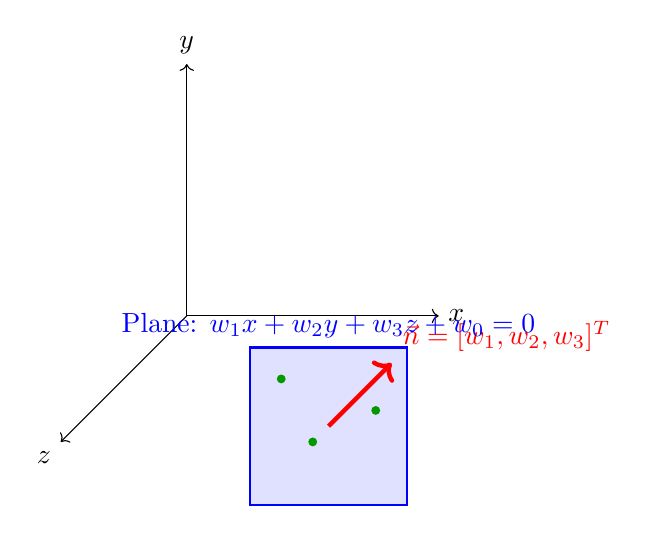
\begin{tikzpicture}[scale=0.8]
    % 3D coordinate system
    \draw[->] (0,0) -- (4,0) node[right] {$x$};
    \draw[->] (0,0) -- (0,4) node[above] {$y$};
    \draw[->] (0,0) -- (-2,-2) node[below left] {$z$};
    
    % Plane
    \fill[blue!20, opacity=0.6] (1,-0.5) -- (3.5,-0.5) -- (3.5,-3) -- (1,-3) -- cycle;
    \draw[blue, thick] (1,-0.5) -- (3.5,-0.5) -- (3.5,-3) -- (1,-3) -- cycle;
    
    % Normal vector
    \draw[->, ultra thick, red] (2.25,-1.75) -- (3.25,-0.75) node[above right] {$\vec{n} = [w_1, w_2, w_3]^T$};
    
    % Points on plane
    \foreach \point in {(1.5,-1), (2,-2), (3,-1.5)} {
        \fill[green!60!black] \point circle (2pt);
    }
    
    % Label
    \node[blue, above] at (2.25,-0.5) {Plane: $w_1x + w_2y + w_3z + w_0 = 0$};
\end{tikzpicture}
\end{center}

\subsection{Hyperplanes in n-Dimensions}

For machine learning problems with many features, we need to generalize beyond 3D visualization.

\begin{definition}[Hyperplane]
A hyperplane in $n$-dimensional space is a linear surface defined by:
\begin{equation}
w_1x_1 + w_2x_2 + w_3x_3 + \cdots + w_nx_n + w_0 = 0
\end{equation}
where:
\begin{itemize}
    \item $x_1, x_2, \ldots, x_n$ are the $n$ features
    \item $w_1, w_2, \ldots, w_n$ are coefficients (also called weights)
    \item $w_0$ is the bias term (intercept in higher dimensions)
\end{itemize}
\end{definition}

\textbf{Dimension of Hyperplane:} A hyperplane in $n$-dimensional space has dimension $n-1$. For example:
\begin{itemize}
    \item In 2D ($n=2$): hyperplane is a line (1D)
    \item In 3D ($n=3$): hyperplane is a plane (2D)
    \item In 100D ($n=100$): hyperplane is a 99-dimensional surface
\end{itemize}

\textbf{Importance in Machine Learning:} The hyperplane equation forms the backbone of many fundamental ML algorithms including:
\begin{itemize}
    \item Linear classifiers
    \item Support Vector Machines (SVM)
    \item Logistic regression
    \item Neural networks (each neuron computes a weighted sum forming a hyperplane)
\end{itemize}

\newpage

\section{Vector Notation and Linear Algebra}

\subsection{Vectors: A More Compact Notation}

The general hyperplane equation $w_1x_1 + w_2x_2 + \cdots + w_nx_n + w_0 = 0$ becomes cumbersome as the number of features increases. Vector notation provides a much more elegant representation.

\begin{definition}[Vector]
A vector is an ordered array of numbers. Conventionally, vectors are written as column vectors:
\begin{equation}
\vec{v} = \begin{bmatrix}
v_1 \\
v_2 \\
\vdots \\
v_n
\end{bmatrix}_{n \times 1}
\end{equation}

The notation $n \times 1$ indicates $n$ rows and 1 column.
\end{definition}

\begin{definition}[Transpose]
The transpose of a vector converts it from a column to a row (or vice versa):
\begin{equation}
\vec{v}^T = [v_1, v_2, \ldots, v_n]_{1 \times n}
\end{equation}

The transpose operation is denoted by the superscript $T$.
\end{definition}

\textbf{Application to Our Problem:}

We can represent the feature vector and weight vector as:
\begin{equation}
\vec{x} = \begin{bmatrix}
x_1 \\
x_2 \\
\vdots \\
x_n
\end{bmatrix}, \quad
\vec{w} = \begin{bmatrix}
w_1 \\
w_2 \\
\vdots \\
w_n
\end{bmatrix}
\end{equation}

Both vectors belong to $\mathbb{R}^n$ (the set of all $n$-dimensional real-valued vectors), while the bias $w_0 \in \mathbb{R}^1$ is a scalar.

\subsection{The Dot Product (Inner Product)}

\begin{definition}[Dot Product]
The dot product (also called inner product or scalar product) of two vectors $\vec{a}$ and $\vec{b}$ is:
\begin{equation}
\vec{a} \cdot \vec{b} = a_1b_1 + a_2b_2 + a_3b_3 + \cdots + a_nb_n = \sum_{i=1}^{n} a_ib_i
\end{equation}

Alternative notation: $\langle \vec{a}, \vec{b} \rangle$ means the same as $\vec{a} \cdot \vec{b}$
\end{definition}

\textbf{Matrix Multiplication Perspective:} The dot product can also be expressed as matrix multiplication:
\begin{equation}
\vec{a} \cdot \vec{b} = \vec{a}^T\vec{b} = [a_1, a_2, \ldots, a_n] \begin{bmatrix}
b_1 \\
b_2 \\
\vdots \\
b_n
\end{bmatrix} = a_1b_1 + a_2b_2 + \cdots + a_nb_n
\end{equation}

\begin{example}[Computing Dot Products]
\textbf{Question:} Find the dot product of $\vec{a} = [1, 2, 3]$ and $\vec{b} = [-1, 2, 5]$.

\textbf{Solution:}
\begin{align}
\vec{a} \cdot \vec{b} &= (1)(-1) + (2)(2) + (3)(5) \\
&= -1 + 4 + 15 \\
&= 18
\end{align}

\textbf{Answer:} 18 (option c)
\end{example}

\subsection{Vector Form of the Hyperplane Equation}

Using vector notation, the lengthy hyperplane equation becomes remarkably concise:

\begin{tcolorbox}[enhanced,breakable,colback=blue!5!white,colframe=blue!75!black,title=Vector Form of Hyperplane]
\textbf{General Form:}
\begin{equation}
w_1x_1 + w_2x_2 + w_3x_3 + \cdots + w_nx_n + w_0 = 0
\end{equation}

\textbf{Vector Form (Equivalent):}
\begin{equation}
\vec{w}^T\vec{x} + w_0 = 0
\end{equation}

This compact representation is universally used in machine learning implementations.
\end{tcolorbox}

\textbf{Expanded View:}
\begin{equation}
\vec{w}^T\vec{x} + w_0 = [w_1, w_2, \ldots, w_n]_{1 \times n} \begin{bmatrix}
x_1 \\
x_2 \\
\vdots \\
x_n
\end{bmatrix}_{n \times 1} + w_0 = 0
\end{equation}

The dimensions work out: $(1 \times n) \times (n \times 1) = (1 \times 1)$ which is a scalar, plus the scalar $w_0$, equals zero.

\newpage

\section{Vector Magnitude and Distance}

\subsection{Norm (Magnitude) of a Vector}

\begin{definition}[Euclidean Norm]
The Euclidean norm (also called magnitude or length) of a vector $\vec{a}$ is defined as:
\begin{equation}
\|\vec{a}\| = \sqrt{\vec{a} \cdot \vec{a}} = \sqrt{a_1^2 + a_2^2 + \cdots + a_n^2}
\end{equation}

This represents the distance from the origin to the point represented by $\vec{a}$.
\end{definition}

\begin{center}
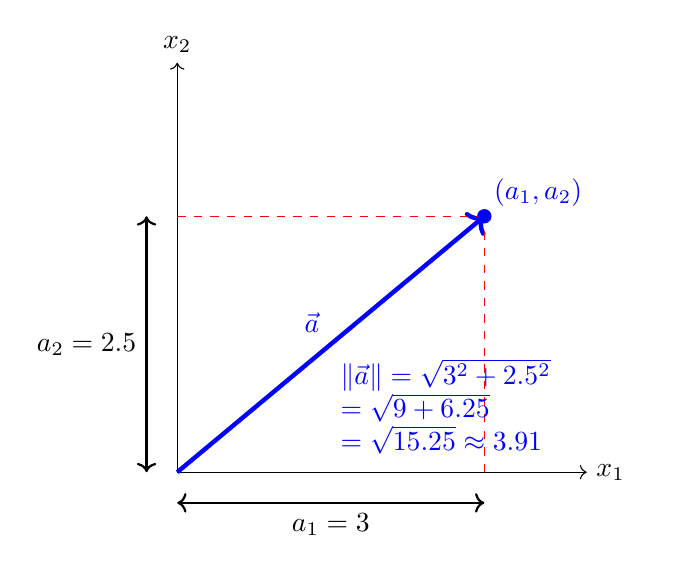
\begin{tikzpicture}[scale=1.3]
    \draw[->] (0,0) -- (4,0) node[right] {$x_1$};
    \draw[->] (0,0) -- (0,4) node[above] {$x_2$};
    
    % Vector
    \draw[->, ultra thick, blue] (0,0) -- (3,2.5) node[midway, above left] {$\vec{a}$};
    
    % Components
    \draw[dashed, red] (3,0) -- (3,2.5);
    \draw[dashed, red] (0,2.5) -- (3,2.5);
    
    % Component labels
    \draw[<->, thick] (0,-0.3) -- (3,-0.3) node[midway, below] {$a_1 = 3$};
    \draw[<->, thick] (-0.3,0) -- (-0.3,2.5) node[midway, left] {$a_2 = 2.5$};
    
    % Magnitude calculation
    \node[blue, below right, text width=4cm, align=left] at (1.5,1.2) {
        $\|\vec{a}\| = \sqrt{3^2 + 2.5^2}$ \\
        $= \sqrt{9 + 6.25}$ \\
        $= \sqrt{15.25} \approx 3.91$
    };
    
    % Point
    \fill[blue] (3,2.5) circle (2pt);
    \node[blue, above right] at (3,2.5) {$(a_1, a_2)$};
\end{tikzpicture}
\end{center}

\begin{example}[Computing Vector Norms]
\textbf{Problem:} Find the norm of $\vec{v} = [3, 4]^T$.

\textbf{Solution:}
\begin{equation}
\|\vec{v}\| = \sqrt{3^2 + 4^2} = \sqrt{9 + 16} = \sqrt{25} = 5
\end{equation}

\textbf{Problem:} Find the norm of $\vec{u} = [1, 2, 2]^T$.

\textbf{Solution:}
\begin{equation}
\|\vec{u}\| = \sqrt{1^2 + 2^2 + 2^2} = \sqrt{1 + 4 + 4} = \sqrt{9} = 3
\end{equation}
\end{example}

\subsection{Angle Between Vectors}

The dot product has a geometric interpretation related to the angle between vectors.

\begin{theorem}[Dot Product and Angle]
For two non-zero vectors $\vec{a}$ and $\vec{b}$, the angle $\phi$ between them satisfies:
\begin{equation}
\cos(\phi) = \frac{\vec{a} \cdot \vec{b}}{\|\vec{a}\| \cdot \|\vec{b}\|}
\end{equation}
\end{theorem}

\textbf{Special Cases:}
\begin{itemize}
    \item If $\vec{a} \cdot \vec{b} = 0$, then $\cos(\phi) = 0$, so $\phi = 90°$ (perpendicular vectors)
    \item If $\vec{a} \cdot \vec{b} > 0$, then $\phi < 90°$ (acute angle)
    \item If $\vec{a} \cdot \vec{b} < 0$, then $\phi > 90°$ (obtuse angle)
\end{itemize}

\begin{center}
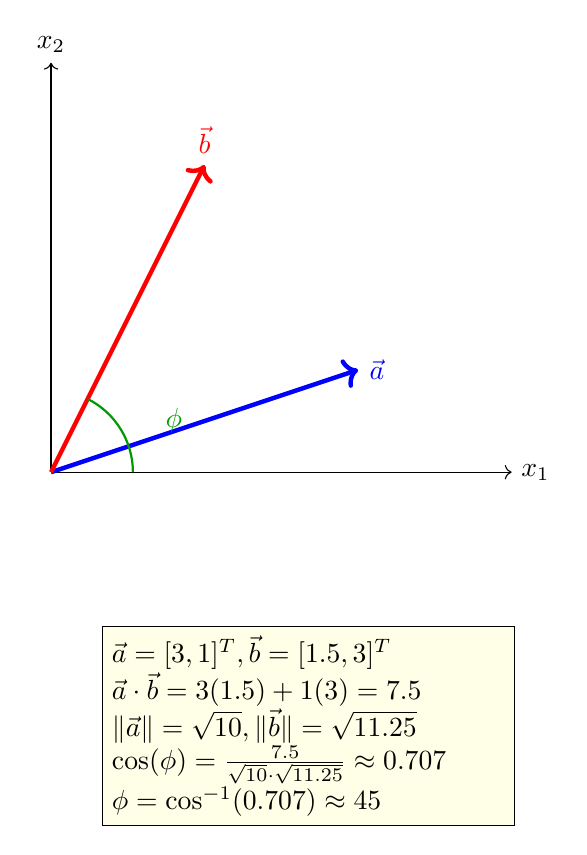
\begin{tikzpicture}[scale=1.3]
    \draw[->] (0,0) -- (4.5,0) node[right] {$x_1$};
    \draw[->] (0,0) -- (0,4) node[above] {$x_2$};
    
    % Vector a
    \draw[->, ultra thick, blue] (0,0) -- (3,1) node[right] {$\vec{a}$};
    
    % Vector b
    \draw[->, ultra thick, red] (0,0) -- (1.5,3) node[above] {$\vec{b}$};
    
    % Angle
    \draw[thick, green!60!black] (0.8,0) arc (0:63:0.8);
    \node[green!60!black] at (1.2,0.5) {$\phi$};
    
    % Calculation box
    \node[draw, fill=yellow!10, text width=5cm, align=left, below right] at (0.5,-1.5) {
        $\vec{a} = [3, 1]^T, \vec{b} = [1.5, 3]^T$ \\
        $\vec{a} \cdot \vec{b} = 3(1.5) + 1(3) = 7.5$ \\
        $\|\vec{a}\| = \sqrt{10}, \|\vec{b}\| = \sqrt{11.25}$ \\
        $\cos(\phi) = \frac{7.5}{\sqrt{10} \cdot \sqrt{11.25}} \approx 0.707$ \\
        $\phi = \cos^{-1}(0.707) \approx 45°$
    };
\end{tikzpicture}
\end{center}

\subsection{Summary: Progression of Equations}

\begin{table}[h!]
\centering
\begin{tabular}{|l|c|c|c|}
\hline
\textbf{Dimension} & \textbf{Space} & \textbf{Equation Form} & \textbf{Vector Form} \\
\hline
2D & Plane & $y = mx + c$ & $ax + by + c = 0$ \\
\hline
3D & Space & $w_1x + w_2y + w_3z + w_0 = 0$ & $\vec{w}^T\vec{x} + w_0 = 0$ \\
\hline
nD & Hyperspace & $\sum_{i=1}^n w_ix_i + w_0 = 0$ & $\vec{w}^T\vec{x} + w_0 = 0$ \\
\hline
\end{tabular}
\end{table}

\textbf{Key Insight:} The vector form $\vec{w}^T\vec{x} + w_0 = 0$ remains unchanged regardless of dimensionality, making it the preferred notation for machine learning algorithms that must work in arbitrary dimensions.

\newpage

\section{Half Spaces and Classification}

\subsection{Dividing Space with a Hyperplane}

A hyperplane doesn't just sit in space - it actively divides the entire space into two distinct regions called half-spaces.

\begin{definition}[Half Spaces]
For a hyperplane defined by $\vec{w}^T\vec{x} + w_0 = 0$, the space is divided into:

\textbf{Positive Half Space:}
\begin{equation}
\{\vec{x} : \vec{w}^T\vec{x} + w_0 > 0\}
\end{equation}

\textbf{Negative Half Space:}
\begin{equation}
\{\vec{x} : \vec{w}^T\vec{x} + w_0 < 0\}
\end{equation}
\end{definition}

\textbf{Classification Using Half Spaces:}

For a new point $\vec{x}_{\text{new}}$, we can classify it by computing $\vec{w}^T\vec{x}_{\text{new}} + w_0$:
\begin{itemize}
    \item If $\vec{w}^T\vec{x}_{\text{new}} + w_0 > 0$ $\rightarrow$ Positive class (e.g., Tangerine)
    \item If $\vec{w}^T\vec{x}_{\text{new}} + w_0 < 0$ $\rightarrow$ Negative class (e.g., Orange)
    \item If $\vec{w}^T\vec{x}_{\text{new}} + w_0 = 0$ $\rightarrow$ Exactly on the boundary
\end{itemize}

\begin{center}
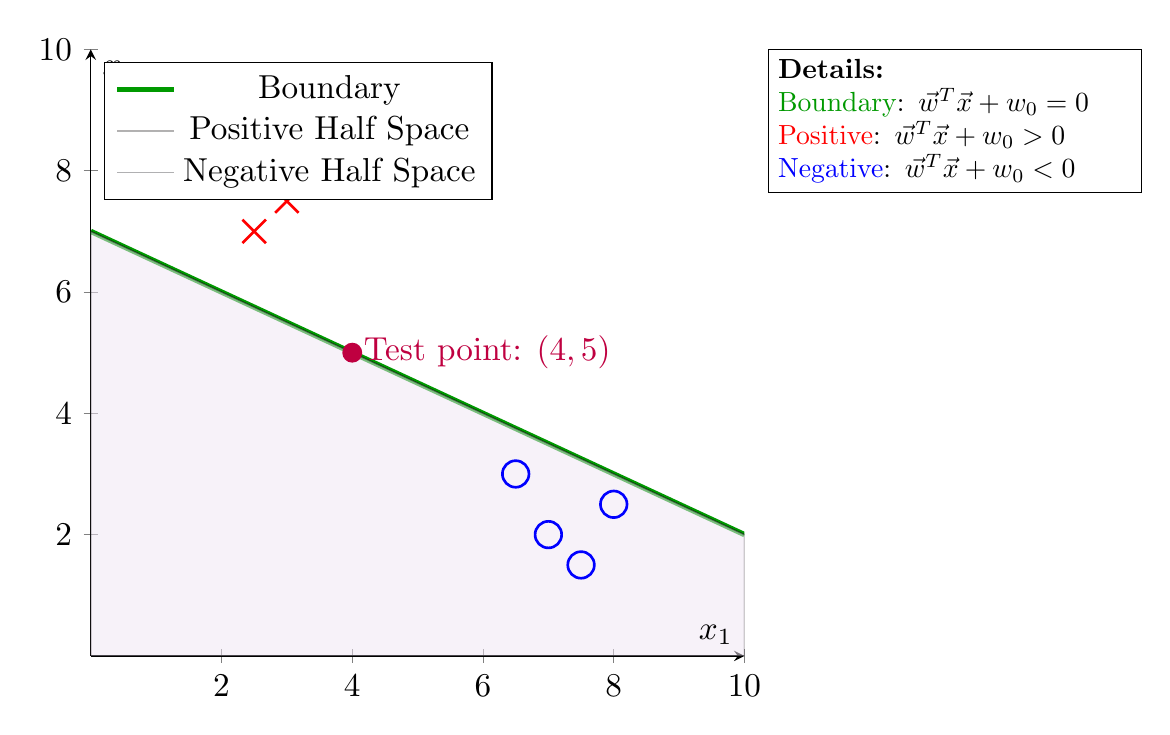
\begin{tikzpicture}[scale=1.2]
    \begin{axis}[
        axis lines=middle,
        xlabel={$x_1$},
        ylabel={$x_2$},
        xmin=0, xmax=10,
        ymin=0, ymax=10,
        width=8.5cm,
        height=8cm,
        legend style={at={(0.02,0.98)}, anchor=north west}
    ]
    
    % Decision boundary
    \addplot[green!60!black, ultra thick, domain=0:10] {-0.5*x + 7};
    \addlegendentry{Boundary}
    
    % Fill half spaces
    \addplot[fill=red!10, opacity=0.3, domain=0:10] {-0.5*x + 7} \closedcycle;
    \addlegendentry{Positive Half Space}
    
    \addplot[fill=blue!10, opacity=0.3, domain=0:10] {-0.5*x + 7} |- (axis cs:10,0) -- (axis cs:0,0) -- cycle;
    \addlegendentry{Negative Half Space}
    
    % Points in positive half space
    \addplot[only marks, mark=x, mark size=5pt, red, thick] coordinates {
        (2, 8) (3, 7.5) (1, 8.5) (2.5, 7)
    };
    
    % Points in negative half space
    \addplot[only marks, mark=o, mark size=4pt, blue, thick] coordinates {
        (7, 2) (8, 2.5) (6.5, 3) (7.5, 1.5)
    };
    
    % Test points
    \fill[purple] (axis cs:4,5) circle (3pt);
    \node[purple, right] at (axis cs:4,5) {Test point: $(4, 5)$};
    
    \end{axis}
    
    % Side Legend for equations
    \node[draw, fill=white, align=left, anchor=north west, text width=4.5cm] at (current axis.north east) [xshift=0.3cm] {
        \textbf{Details:}\\
        \textcolor{green!60!black}{Boundary}: $\vec{w}^T\vec{x} + w_0 = 0$\\
        \textcolor{red}{Positive}: $\vec{w}^T\vec{x} + w_0 > 0$\\
        \textcolor{blue}{Negative}: $\vec{w}^T\vec{x} + w_0 < 0$
    };
\end{tikzpicture}
\end{center}

\begin{example}[Half Space Classification]
\textbf{Given:} Decision boundary $2x_1 + x_2 - 10 = 0$ (equivalently, $\vec{w} = [2, 1]^T, w_0 = -10$)

\textbf{Classify:} Point $(4, 5)$

\textbf{Solution:}
\begin{align}
\vec{w}^T\vec{x} + w_0 &= 2(4) + 1(5) - 10 \\
&= 8 + 5 - 10 \\
&= 3 > 0
\end{align}

Since the result is positive, the point $(4, 5)$ belongs to the positive half space.

\textbf{Classify:} Point $(1, 2)$

\textbf{Solution:}
\begin{align}
\vec{w}^T\vec{x} + w_0 &= 2(1) + 1(2) - 10 \\
&= 2 + 2 - 10 \\
&= -6 < 0
\end{align}

Since the result is negative, the point $(1, 2)$ belongs to the negative half space.
\end{example}

\newpage

\section{The "Best" Decision Boundary}

\subsection{What Makes a Boundary "Best"?}

We've established that we can draw lines to separate classes, but there are infinitely many lines that could separate two clusters. The crucial question is: which line should we choose?

\begin{center}
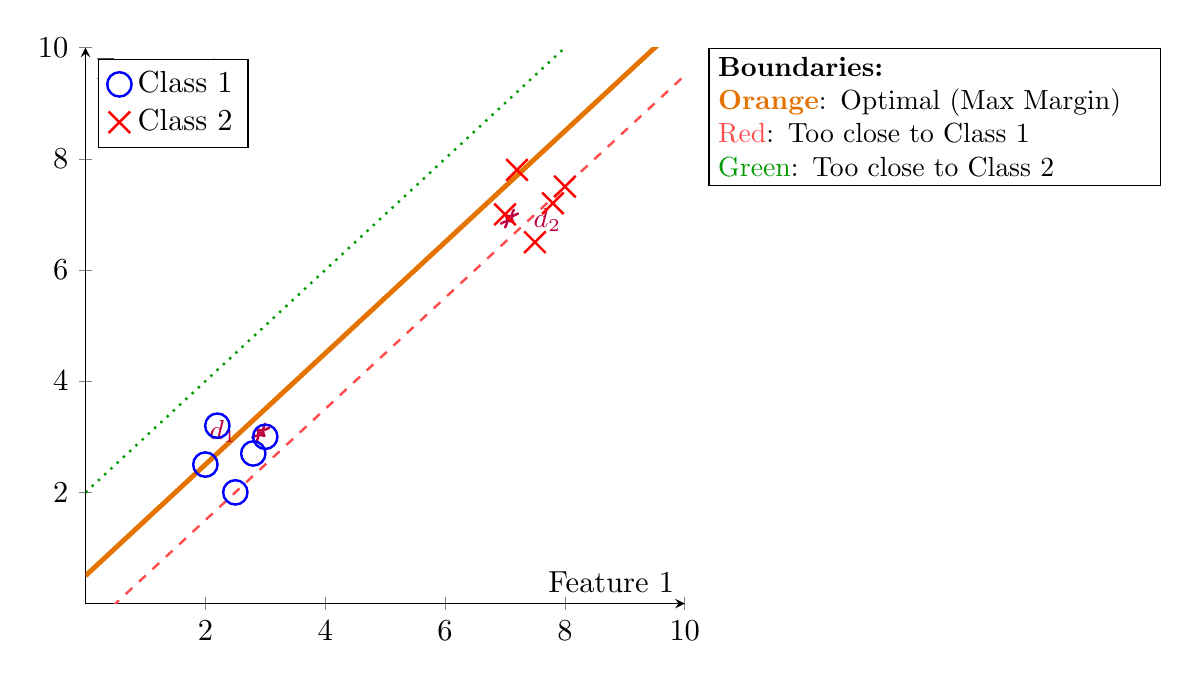
\begin{tikzpicture}[scale=1.1]
    \begin{axis}[
        axis lines=middle,
        xlabel={Feature 1},
        ylabel={Feature 2},
        xmin=0, xmax=10,
        ymin=0, ymax=10,
        width=8.5cm,
        height=8cm,
        legend style={at={(0.02,0.98)},anchor=north west}
    ]
    
    % Class 1 points
    \addplot[only marks, mark=o, mark size=4pt, blue, thick] coordinates {
        (2, 2.5) (2.5, 2) (3, 3) (2.2, 3.2) (2.8, 2.7)
    };
    
    % Class 2 points
    \addplot[only marks, mark=x, mark size=5pt, red, thick] coordinates {
        (7, 7) (7.5, 6.5) (8, 7.5) (7.2, 7.8) (7.8, 7.2)
    };
    
    % Three candidate boundaries
    \addplot[red!70, thick, dashed, domain=0:10] {x - 0.5};
    
    \addplot[orange!90!black, ultra thick, domain=0:10] {x + 0.5};
    
    \addplot[green!60!black, thick, dotted, domain=0:10] {x + 2};
    
    % Distance indicators for orange line
    \draw[<->, purple, thick] (axis cs:3,3) -- (axis cs:2.85,3.15);
    \node[purple, left, font=\small] at (axis cs:2.7,3.1) {$d_1$};
    
    \draw[<->, purple, thick] (axis cs:7,7) -- (axis cs:7.15,6.85);
    \node[purple, right, font=\small] at (axis cs:7.3,6.9) {$d_2$};

    % Legend with explanations
    \legend{Class 1, Class 2}
    
    \end{axis}
    
    % Side Legend Node - Moved OUTSIDE the axis environment
    \node[draw, fill=white, align=left, anchor=north west, text width=5.5cm] at (current axis.north east) [xshift=0.3cm] {
        \textbf{Boundaries:}\\
        \textcolor{orange!90!black}{\textbf{Orange}}: Optimal (Max Margin)\\
        \textcolor{red!70}{Red}: Too close to Class 1\\
        \textcolor{green!60!black}{Green}: Too close to Class 2
    };
\end{tikzpicture}
\end{center}

\subsection{The Margin Principle}

\begin{tcolorbox}[enhanced,breakable,colback=green!5!white,colframe=green!75!black,title=Optimal Decision Boundary Principle]
The \textbf{best} decision boundary is the one that maximizes the minimum distance to points from both classes. This is called maximizing the \textbf{margin}.

\textbf{Why?} A larger margin provides:
\begin{itemize}
    \item Greater robustness to small variations in data
    \item Better generalization to new, unseen examples
    \item Lower sensitivity to measurement noise
    \item Improved confidence in predictions near the boundary
\end{itemize}
\end{tcolorbox}

\textbf{Mathematical Formulation:}

The optimal boundary $\vec{w}^*$ and $w_0^*$ solve:
\begin{equation}
\max_{\vec{w}, w_0} \left\{ \min_{i=1,\ldots,n} \text{distance}(\vec{x}_i, \text{boundary}) \right\}
\end{equation}

This optimization problem requires us to:
\begin{enumerate}
    \item Compute distances from points to the boundary
    \item Find the configuration that maximizes the smallest such distance
\end{enumerate}

\subsection{Distance Computation Preview}

To find the optimal boundary, we need a formula for the distance from a point to a hyperplane. This is where our linear algebra tools become essential.

\textbf{Distance from point $\vec{x}_i$ to hyperplane $\vec{w}^T\vec{x} + w_0 = 0$:}
\begin{equation}
d = \frac{|\vec{w}^T\vec{x}_i + w_0|}{\|\vec{w}\|}
\end{equation}

The derivation of this formula requires understanding:
\begin{itemize}
    \item Vector projections
    \item Perpendicular distances
    \item Geometric properties of dot products
\end{itemize}

These topics will be covered in depth in subsequent lectures focusing on linear algebra and vector calculus.

\newpage

\section{Forms of Line Equations: Complete Reference}

\subsection{Five Standard Forms}

Different forms of line equations are useful in different contexts. Here's a comprehensive overview:

\begin{enumerate}
    \item \textbf{Slope-Intercept Form:}
    \begin{equation}
    y = mx + c
    \end{equation}
    \textbf{Use:} When slope and intercept are known; most intuitive form.
    
    \item \textbf{Point-Slope Form:}
    \begin{equation}
    y - y_1 = m(x - x_1)
    \end{equation}
    \textbf{Use:} When you know one point $(x_1, y_1)$ and the slope $m$.
    
    \item \textbf{Two-Point Form:}
    \begin{equation}
    y - y_1 = \frac{y_2 - y_1}{x_2 - x_1}(x - x_1)
    \end{equation}
    \textbf{Use:} When you know two points $(x_1, y_1)$ and $(x_2, y_2)$ on the line.
    
    \item \textbf{Intercept Form:}
    \begin{equation}
    \frac{x}{a} + \frac{y}{b} = 1
    \end{equation}
    \textbf{Use:} When x-intercept is $a$ and y-intercept is $b$.
    
    \item \textbf{General Form:}
    \begin{equation}
    ax + by + c = 0
    \end{equation}
    \textbf{Use:} Standard form; generalizes to hyperplanes; used in ML algorithms.
\end{enumerate}

\begin{example}[Converting Between Forms]
\textbf{Given:} Two points $(2, 3)$ and $(4, 7)$

\textbf{Find:} All five forms of the line equation.

\textbf{Solution:}

\textit{Step 1: Find slope}
\begin{equation}
m = \frac{7 - 3}{4 - 2} = \frac{4}{2} = 2
\end{equation}

\textit{Step 2: Find y-intercept using point $(2, 3)$}
\begin{equation}
3 = 2(2) + c \implies c = -1
\end{equation}

\textbf{Forms:}
\begin{enumerate}
    \item Slope-intercept: $y = 2x - 1$
    \item Point-slope: $y - 3 = 2(x - 2)$ or $y - 7 = 2(x - 4)$
    \item Two-point: $y - 3 = \frac{7-3}{4-2}(x - 2) = 2(x - 2)$
    \item General: $2x - y - 1 = 0$
    \item Intercept: $\frac{x}{0.5} + \frac{y}{-1} = 1$ (x-intercept is 0.5, y-intercept is -1)
\end{enumerate}
\end{example}

\newpage

\section{Comprehensive Worked Examples}

\subsection{Example 1: Complete Classification Pipeline}

\begin{example}[End-to-End Fruit Classification]
\textbf{Given Dataset:}

\begin{center}
\begin{tabular}{|c|c|c|}
\hline
\textbf{Diameter} & \textbf{Weight} & \textbf{Fruit} \\
\hline
7 & 65 & O \\
8 & 75 & O \\
9 & 80 & O \\
10 & 95 & T \\
11 & 100 & T \\
12 & 105 & T \\
\hline
\end{tabular}
\end{center}

\textbf{Task:} Find a linear decision boundary to separate oranges from tangerines.

\textbf{Solution Approach:}

\textit{Step 1: Visualize the data}

Plot the points on a Diameter-Weight plane. Visual inspection suggests a line with negative slope could separate the classes.

\textit{Step 2: Propose a boundary}

Let's try the line: $W = -3D + 115$ or in general form: $3D + W - 115 = 0$

In vector notation with $\vec{x} = [D, W]^T$:
\begin{equation}
\vec{w}^T\vec{x} + w_0 = 3D + 1W - 115 = 0
\end{equation}

So $\vec{w} = [3, 1]^T$ and $w_0 = -115$.

\textit{Step 3: Test all points}

For Oranges (should be in negative half space):
\begin{align}
(7, 65): \quad 3(7) + 65 - 115 &= -29 < 0 \quad (Correct) \\
(8, 75): \quad 3(8) + 75 - 115 &= -16 < 0 \quad (Correct) \\
(9, 80): \quad 3(9) + 80 - 115 &= -8 < 0 \quad (Correct)
\end{align}

For Tangerines (should be in positive half space):
\begin{align}
(10, 95): \quad 3(10) + 95 - 115 &= 10 > 0 \quad (Correct) \\
(11, 100): \quad 3(11) + 100 - 115 &= 16 > 0 \quad (Correct) \\
(12, 105): \quad 3(12) + 105 - 115 &= 26 > 0 \quad (Correct)
\end{align}

\textbf{Result:} This boundary perfectly separates all training points!
\end{example}

\subsection{Example 2: Understanding Misclassification}

\begin{example}[Handling Imperfect Boundaries]
\textbf{Modified Dataset:} Add a noisy point: $(9, 98, O)$ - an unusually heavy orange.

\textbf{Analysis with previous boundary $3D + W - 115 = 0$:}
\begin{equation}
3(9) + 98 - 115 = 27 + 98 - 115 = 10 > 0
\end{equation}

This orange would be misclassified as a tangerine because it falls in the positive half space!

\textbf{Options:}
\begin{enumerate}
    \item \textbf{Adjust the boundary:} Find a new line that correctly classifies this point (may misclassify others)
    \item \textbf{Accept the error:} Recognize that perfect separation isn't always possible with linear boundaries
    \item \textbf{Use complex boundaries:} Consider non-linear decision boundaries (covered in advanced ML)
\end{enumerate}

This example illustrates that real-world classification often involves trade-offs between different types of errors.
\end{example}

\subsection{Example 3: IPL Match Prediction}

\begin{example}[Cricket Match Outcome Prediction]
\textbf{Scenario:} A marketing company runs ads during IPL matches. They want to stop advertising early if a match is already decided to save costs.

\textbf{Features:}
\begin{itemize}
    \item $x_1$: Runs scored by batting team
    \item $x_2$: Overs completed
\end{itemize}

\textbf{Target:} Win (W) or Loss (L)

\textbf{Sample Data:}

\begin{center}
\begin{tabular}{|c|c|c|}
\hline
\textbf{Runs} & \textbf{Overs} & \textbf{Outcome} \\
\hline
45 & 6 & L \\
78 & 10 & W \\
52 & 8 & L \\
95 & 12 & W \\
110 & 15 & W \\
60 & 10 & L \\
\hline
\end{tabular}
\end{center}

\textbf{Visualization Insight:} When plotted, winning matches (W) cluster in the upper-right region (high runs, moderate overs), while losing matches (L) cluster in the lower-left (low runs). A decision boundary can separate these regions.

\textbf{Business Application:} Once the boundary is learned, the system can predict in real-time: "If current position is in the win region with high confidence, continue ads; if in loss region, stop ads to save budget."
\end{example}

\newpage

\section{Practice Problems and Exercises}

\begin{problem}[Line Equations]
For each set of information, write the equation of the line in both slope-intercept and general form:
\begin{enumerate}[label=(\alph*)]
    \item Slope $m = 3$, y-intercept $c = -2$
    \item Passes through $(1, 4)$ and $(3, 10)$
    \item x-intercept $= 5$, y-intercept $= -3$
    \item Parallel to $2x + 3y - 7 = 0$ and passes through $(0, 4)$
\end{enumerate}
\end{problem}

\begin{problem}[Parallel and Perpendicular Lines]
\begin{enumerate}[label=(\alph*)]
    \item Find the equation of a line parallel to $y = 4x - 1$ passing through $(2, 5)$
    \item Find the equation of a line perpendicular to $y = -\frac{1}{3}x + 2$ passing through the origin
    \item Determine whether the lines $2x - 3y + 5 = 0$ and $3x + 2y - 1 = 0$ are parallel, perpendicular, or neither
\end{enumerate}
\end{problem}

\begin{problem}[Vector Operations]
Given $\vec{a} = [2, -1, 3]^T$, $\vec{b} = [1, 4, -2]^T$, and $\vec{c} = [-3, 0, 5]^T$:
\begin{enumerate}[label=(\alph*)]
    \item Compute $\vec{a} \cdot \vec{b}$
    \item Compute $\|\vec{a}\|$ and $\|\vec{b}\|$
    \item Find the angle between $\vec{a}$ and $\vec{b}$
    \item Verify that $(\vec{a} + \vec{b}) \cdot \vec{c} = \vec{a} \cdot \vec{c} + \vec{b} \cdot \vec{c}$
\end{enumerate}
\end{problem}

\begin{problem}[Half Space Classification]
Consider the decision boundary $2x_1 - 3x_2 + 6 = 0$.
\begin{enumerate}[label=(\alph*)]
    \item Classify the point $(3, 4)$
    \item Classify the point $(0, 0)$
    \item Find a point that lies exactly on the boundary
    \item If class A is in the positive half space and class B is in the negative half space, which class does $(5, 2)$ belong to?
\end{enumerate}
\end{problem}

\begin{problem}[Feature Space Visualization]
You are building a classifier to predict if a student will pass or fail based on hours studied and sleep hours.

\textbf{Dataset:}
\begin{center}
\begin{tabular}{|c|c|c|}
\hline
\textbf{Study Hours} & \textbf{Sleep Hours} & \textbf{Result} \\
\hline
2 & 4 & Fail \\
5 & 7 & Pass \\
3 & 5 & Fail \\
7 & 6 & Pass \\
8 & 8 & Pass \\
1 & 3 & Fail \\
\hline
\end{tabular}
\end{center}

\begin{enumerate}[label=(\alph*)]
    \item Sketch the scatter plot
    \item Propose a reasonable linear decision boundary
    \item Write the equation of your boundary in vector form
    \item Classify a student with 4 study hours and 6 sleep hours
\end{enumerate}
\end{problem}

\begin{problem}[Multi-class Extension]
Suppose we want to classify fruits into three categories: Small (S), Medium (M), Large (L) based on diameter and weight.
\begin{enumerate}[label=(\alph*)]
    \item How many decision boundaries would we need minimum?
    \item Sketch a possible configuration of boundaries
    \item What happens if the boundaries intersect? Is this problematic?
\end{enumerate}
\end{problem}

\newpage

\section{Summary and Next Steps}

\subsection{Key Concepts Covered}

\begin{tcolorbox}[enhanced,breakable,colback=yellow!10!white,colframe=orange!75!black,title=Module 1 Summary]

\textbf{1. Machine Learning Fundamentals:}
\begin{itemize}
    \item Machine learning enables automated decision-making from data
    \item Classification involves finding decision boundaries between classes
    \item Geometric visualization helps build intuition before formal math
\end{itemize}

\textbf{2. Feature Engineering:}
\begin{itemize}
    \item Features are the measurable attributes used for prediction
    \item Not all features are equally informative
    \item Feature selection requires domain knowledge
\end{itemize}

\textbf{3. Linear Boundaries:}
\begin{itemize}
    \item Lines in 2D, planes in 3D, hyperplanes in nD
    \item Multiple equivalent forms: slope-intercept, general, vector
    \item Vector form $\vec{w}^T\vec{x} + w_0 = 0$ generalizes to any dimension
\end{itemize}

\textbf{4. Optimization Goal:}
\begin{itemize}
    \item Best boundary maximizes margin between classes
    \item Requires computing distances to hyperplanes
    \item Machine learning algorithms automate this search
\end{itemize}

\textbf{5. Linear Algebra Tools:}
\begin{itemize}
    \item Vectors provide compact notation for high-dimensional data
    \item Dot products enable distance and angle calculations
    \item Norms measure vector magnitudes
\end{itemize}
\end{tcolorbox}

\begin{example}[Calculating Distance to Boundary]
\textbf{Problem:} Calculate the perpendicular distance from point $P(2, 4)$ to the decision boundary line $3x + 4y - 12 = 0$.

\textbf{Solution Steps:}
\begin{enumerate}
    \item Identify the parameters from the line equation $ax + by + c = 0$:
    $$ a = 3, \quad b = 4, \quad c = -12 $$
    \item Identify the point coordinates $(x_0, y_0)$:
    $$ x_0 = 2, \quad y_0 = 4 $$
    \item Apply the distance formula:
    $$ d = \frac{|ax_0 + by_0 + c|}{\sqrt{a^2 + b^2}} $$
    \item Substitute the values:
    \begin{align*}
    d &= \frac{|3(2) + 4(4) - 12|}{\sqrt{3^2 + 4^2}} \\
    &= \frac{|6 + 16 - 12|}{\sqrt{9 + 16}} \\
    &= \frac{|10|}{\sqrt{25}} \\
    &= \frac{10}{5} = 2
    \end{align*}
\end{enumerate}
\textbf{Answer:} The distance is 2 units.
\end{example}

\subsection{Practical Skills to Develop}

To reinforce these concepts, practice the following:

\begin{enumerate}
    \item \textbf{Visualization:} Use Desmos or Python (matplotlib) to plot datasets and experiment with different decision boundaries
    \item \textbf{Vector Calculations:} Become fluent with dot products, norms, and vector arithmetic
    \item \textbf{Form Conversion:} Practice converting between different line equation forms quickly
    \item \textbf{Geometric Intuition:} Train yourself to visualize high-dimensional problems using 2D/3D analogies
\end{enumerate}

\subsection{Connection to Real ML Algorithms}

The concepts introduced here directly map to production machine learning algorithms:

\begin{center}
\begin{tabular}{|p{4cm}|p{10cm}|}
\hline
\textbf{Concept} & \textbf{ML Algorithm} \\
\hline
Linear decision boundary & Linear SVM, Perceptron, Logistic Regression \\
\hline
Maximizing margin & Support Vector Machines (SVM) \\
\hline
Half-space classification & All linear classifiers \\
\hline
Hyperplane in nD & Neural network layers (each neuron is a hyperplane) \\
\hline
Finding optimal $\vec{w}$ & Gradient descent, backpropagation \\
\hline
\end{tabular}
\end{center}


\end{document}